%!TEX root = etdrtemplate.tex

\cleardoublepage


\chapter{Background}
\label{background}

This chapter is a brief introduction of all technologies and tools used in this thesis. There are: AADL modeling language, BLESS (AADL annex language), SPARK Ada programming language and its verification tools. There is also overview of the context in which this work has been made: Integrated Clinical Environment standard (ICE) and PCA Pump (ICE compliant device). This is followed by main topic of the thesis: code generation from AADL and analysis of existing AADL translators (Ocarina, RAMSES).



\section{Integrated Clinical Environment}
\label{background:ice}
%http://santos.cis.ksu.edu/MDCF/doc/ICE-Motivation.pdf

Idea of "Integrated Clinical Environment" (ICE) was initiated by Dr. Julian Goldman from Center for Integration of Medicine \& Innovative Technology. The main idea is to create environment of different medical devices working together. It allows clinician and software system to make decisions based not only on output from one device, but from all of them together. ICE purpose is to solve current issues with medical devices usually operate independently. It requires more human attention and control through checking output of every device manually and then making decision. ICE will make it easier, by introducing alarms, which can not only indicate problem but also interact with other devices. E.g. when PCA Pump infuse some drug to patient's vein and Pulse Oximeter detects low oxygen level, ICE can coordinate PCA Pump shutdown. PCA Pump, more precisely: drug which is being dosed by it, might be the cause of low oxygen level. In worst case scenario it may cause patient's death.

Moreover, ICE comprises components that may be implemented by different vendors. Such components are medical devices and applications to supervise them. Figure \ref{figure:ice} presents high overview of ICE system. Medical devices (PCA Pump, Respiratory Rate Monitor and Pulse Oximeter) are connected to the system. All of them are monitored and controlled. There is communication between devices and ICE, in order to exchange data between them and Electronic Medical Record (EMR) Database. Informations in EMR comprises drug library, patient's medical records, monitoring logs etc. It enable ICE to make decisions such as PCA Pump shutdown.

\begin{figure}[ht]%t=top, b=bottom, h=here
    \begin{center}
    	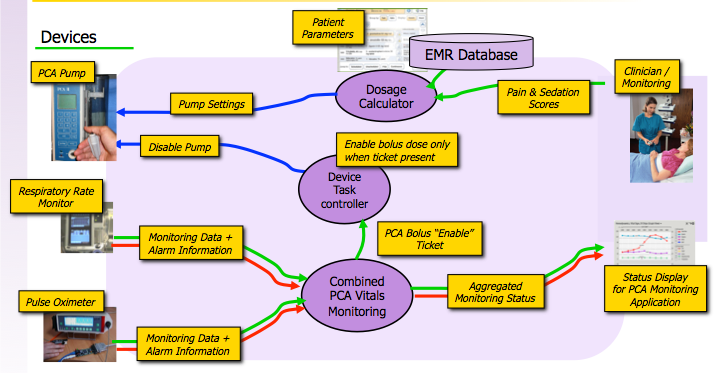
\includegraphics[height=3.5in]{figures/ice.png}
    	\caption{ICE Closed Loop Control}    	
    \end{center}
    \label{figure:ice}
\end{figure}

[ADD MORE INFORMATION?]


\section{Medical Device Coordination Framework}
\label{background:mdcf}
%http://santos.cis.ksu.edu/MDCF/doc/MDCF-Tutorial-Overview.pdf

Medical Device Coordination Framework (MDCF), jointly developed by SAnToS lab (Kansas State University) and University of Pennsylvania is prototype implementation of ICE. It is an open, experimental platform to bring together academic researchers, industry vendors, and government regulators. Project is response to request from Food and Drug Administration (FDA) to build a prototype of ICE. Medical Devices, which are ICE compliant can be connected to MDCF. MDCF enables Medical Devices interoperability. MDCF is designed to illustrate by example the issues related to functional concepts, safety, security, verification and certification. 

The goals of MDCF project comprises:
\begin{itemize}
	\item Open source infrastructure
	\item Meet performance requirements of realistic clinical scenarios
	\item Provide middleware with reliability, real-time, security
	\item Provide an effective app programming model and development environment with integrated verification/validation support and construction of regulatory artifacts
	\item Support evaluation of device interfacing concepts
	\item Illustrate how to support real and mock devices
	\item Illustrate envisioned regulatory oversight and 3rd party certification
\end{itemize}

In this thesis, part of penultimate point will be illustrated. For now, MDCF use only mock devices, which are Java desktop applications. PCA Pump Prototype aim to be first real-device.

MDCF uses publish-subscribe architecture for communication between components: apps and devices. Figure \ref{figure:mdcf} presents MDCF structure. Devices, like PCA Pump, are clients. MDCF Server is integration layer which comprises Core and applications working in top of it. \cite{MDCF:Paper}.

\begin{figure}[ht]%t=top, b=bottom, h=here
    \begin{center}
    	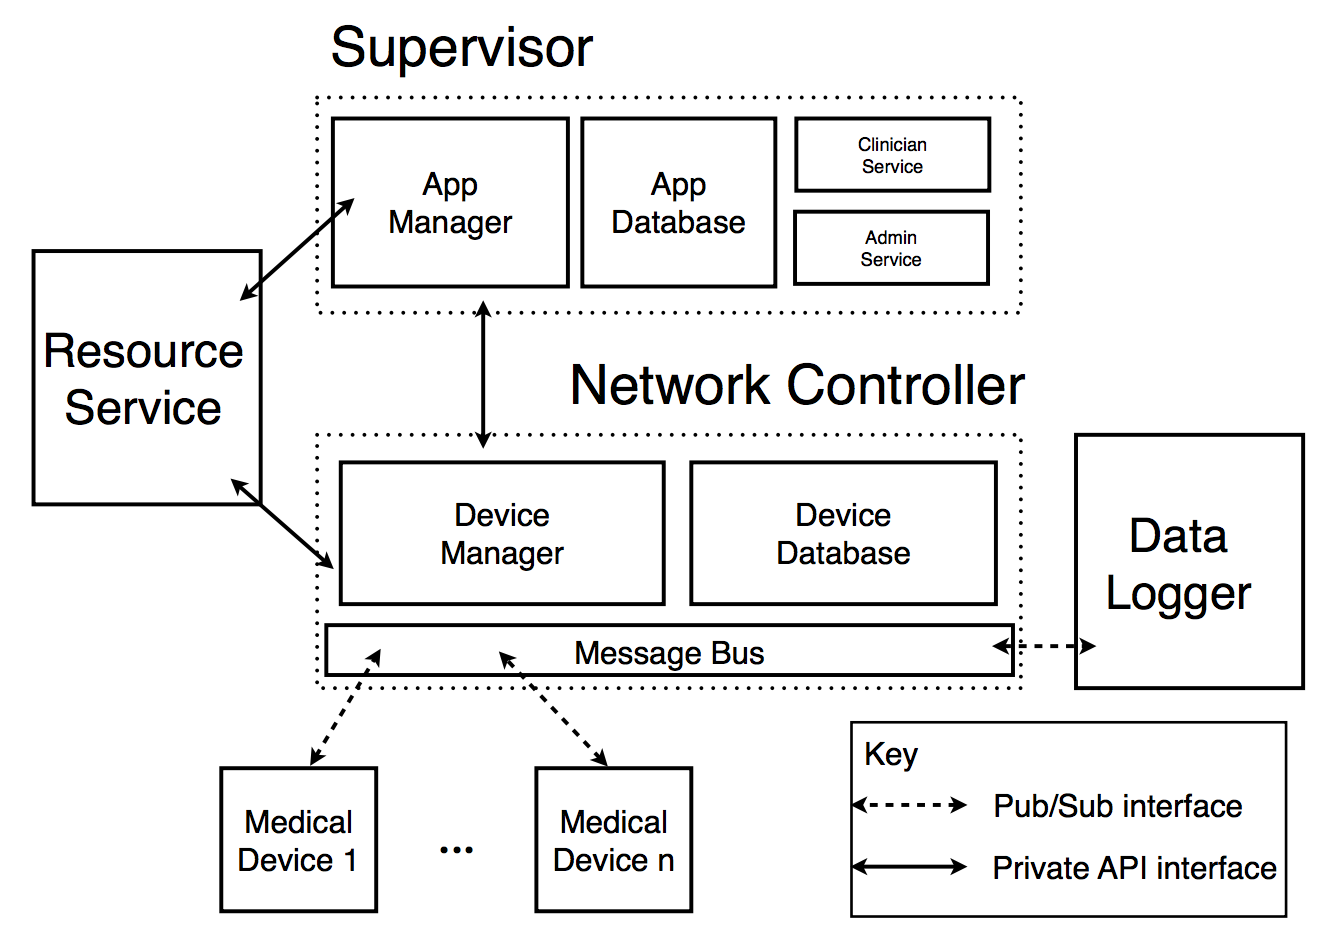
\includegraphics[height=3in]{figures/mdcf.png}
    	\caption{MDCF architecture and example app virtual machine (lower right)}    	
    \end{center}
    \label{figure:mdcf}
\end{figure}

[ADD MORE INFORMATION?]



\section{AADL}
\label{background:aadl}

AADL stands for Architecture Analysis \& Design Language. It is used to model embedded and real-time systems. AADL allows for the description of both software and hardware parts of a system. It can be used not only for design phase of software development process, but also for analysis, verification or code generation.

AADL has its roots in DARPA \footnote{http://www.darpa.mil} funded research. The first version (1.0) was approved in 2004 under technical leadership of Peter Feiler\footnote{http://wiki.sei.cmu.edu/aadl/index.php/The\_Story\_of\_AADL/}. AADL is develop by SAE AADL committee\footnote{https://wiki.sei.cmu.edu/aadl/index.php/Main\_Page}. AADL version 2.0 was published in January 2009. The most recent version (2.1) was published in September 2012\footnote{https://wiki.sei.cmu.edu/aadl/index.php/Standardization}.

AADL is a language for Model-Based Engineering \cite{AadlBook}. It can be represented in textual and graphical form. There are tools (like Osate, see section \ref{background:aadl:osate}), which transforms textual representation into graphical. There is also possibility to represent AADL in XML (using 3rd party tools). 

\begin{wrapfigure}{r}{0.3\textwidth}
  \begin{center}
    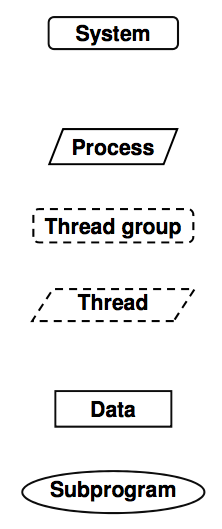
\includegraphics[width=0.2\textwidth]{figures/aadl-app-components.png}
  \end{center}
  \caption{AADL Application Software Components}
  \label{figure:aadl_app_software_components}
\end{wrapfigure}

Execution Platform Components and Devices:
\begin{itemize}
	\item Processor / Virtual Processor - Provides thread scheduling and execution services
	\item Memory - provides storage for data and source code
	\item Bus / Virtual Bus - provides physical/logical connectivity between execution platform components
	\item Device - interface to external environment
\end{itemize}

Application Software Components of AADL:
\begin{itemize}
	\item System - hierarchical organization of components
	\item Process - protected address space
	\item Thread group - logical organization of threads
	\item Thread - a schedulable unit of concurrent execution
	\item Data - potentially sharable data
	\item Subprogram - callable unit of sequential code
\end{itemize}

Graphical representation of Application Software Components is depicted on figure \ref{figure:aadl_app_software_components}.

An example AADL model Thermometer is shown in graphical representation, in figure \ref{figure:patient_thermometer} and in textual representation, in listing \ref{listing:patient_thermometer}.

\begin{figure}[ht]%t=top, b=bottom, h=here
    \begin{center}
    	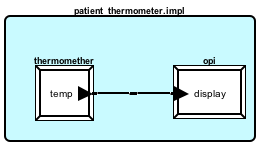
\includegraphics[height=1.5in]{figures/patient_thermometer.png}
    	\caption{AADL model of simple thermometer}
    \end{center}
    \label{figure:patient_thermometer}
\end{figure}

\singlespacing
\begin{lstlisting}[language=aadl, frame=single, gobble=0, caption={AADL model of simple thermometer}, label={listing:patient_thermometer}]
	package Thermometer
	public
	with Base_Types;
		system patient_thermometer
		end patient_thermometer;

		system implementation patient_thermometer.impl
		subcomponents
			thermomether : device thermometer_device.impl;
			opi : device operator_interface.impl;
		connections
			tdn : port thermomether.temp -> opi.display;
		end patient_thermometer.impl;

		device operator_interface
		features
			display : in data port Base_Types::Integer;
		end operator_interface;

		device implementation operator_interface.impl
		end operator_interface.impl;

		device thermometer_device
		features
			temp : out data port Base_Types::Integer;
		end thermometer_device;

		device implementation thermometer_device.impl
		end thermometer_device.impl;
	end Thermometer;
\end{lstlisting} 
\doublespacing
%another example: https://wiki.sei.cmu.edu/aadl/images/7/73/AADLV2Overview-AADLUserDay-Feb_2010.pdf (slide 16)

Recently AADL becomes a new market standard. There are lots of tools for AADL models analysis, such as: STOOD\footnote{http://www.ellidiss.com/products/stood}, ADELE\footnote{https://wiki.sei.cmu.edu/aadl/index.php/Adele}, Cheddar\footnote{http://beru.univ-brest.fr/~singhoff/cheddar}, AADLInspector\footnote{http://www.ellidiss.com/products/aadl-inspector} or Ocarina\footnote{http://www.openaadl.org}.

What is important, AADL is for architectural description. It should not be compared with UML suites, which allows to link with source code.

AADL can be extended with the following methods:
\begin{itemize}
	\item user-defined properties: user can extend the set of applicable properties and add their own to specify their own requirements
	\item {language annexes (the core language is enhanced by annex languages that enrich the architecture description. For now, the following annexes have been defined):
		\begin{itemize}
			\item Behavior annex: add components behavior with state machines
			\item Error-model annex: specifies fault and propagation concerns
			\item ARINC653 annex: defines modelling patterns for modelling avionics system
			\item Data-Model annex: describes the modelling of specific data constraint with AADL
		\end{itemize}
		}
\end{itemize}

BLESS (described in section \ref{background:bless}) is AADL behavior annex language.

More details about AADL can be found in Peter Feiler's book "Model-Based Engineering with AADL" \cite{AadlBook}.


\subsection{OSATE}
\label{background:aadl:osate}

Open Source AADL Tool Environment (OSATE) is a set of plug-ins on top of the open-source Eclipse platform. It provides a tool set for front-end processing of AADL models. OSATE is developed mainly by SEI (Software Engineering Institute - CMU)\footnote{http://www.aadl.info/aadl/currentsite/tool/osate.html}. Latest available version of OSATE in the time when this work was published is OSATE2\footnote{https://wiki.sei.cmu.edu/aadl/index.php/Osate\_2}. 

OSATE relies on EMF, UML2 and XText. It comprises e.g. AADL project wizard, AADL Navigator or AADL syntax. OSATE enables conversion of AADL in textual representation into graphical. There are also plug-ins for OSATE, like BLESS\footnote{http://bless.santoslab.org/node/5} or OCARINA\footnote{http://libre.adacore.com/tools/ocarina/}.



\section{BLESS}
\label{background:bless}
BLESS (Behavior Language for Embedded Systems with Software) is AADL annex sublanguage defining behavior of components. The goal of BLESS is automatically-checked correctness proofs of AADL models of embedded electronic systems with software.

BLESS contains three AADL annex sublanguages:
\begin{itemize} \itemsep1pt \parskip0pt \parsep0pt
	\item Assertion - it can be attached individually to AADL features (e.g. ports)
	\item subBLESS - can be attached only to subprograms; it has only value transformations and Assertions without time expressions
	\item BLESS - it can be attached to AADL thread, device or system components; it contains states, transitions, timeouts, actions, events and Assertions with time expressions...
\end{itemize}

BLESS annex subclauses can be added to AADL models transparently to other uses of the system architecture. It includes a verification-condition (VC) generation framework and an accompanying proof tool that enables engineers to prove VCs via proof scripts build from system axioms and rules from a user-customizable rule library. \cite{Bless:Paper}

The BLESS tool framework is implemented as a publicly available open source plug-in to the Eclipse-based OSATE environment for AADL (mentioned in section \ref{background:aadl:osate}), and includes and editor for BLESS specifications and an environment operating the BLESS proof engine. \cite{Bless:Paper}

Some BLESS constructs can be translated into SPARK contracts, which is part of this thesis. Additionally, BLESS allows to model behavior of components, which is not done in this thesis, but it is a future work.

[MORE DETAILS? EXAMPLES?]



\section{SPARK Ada}
\label{background:spark}

%http://www.cs.swan.ac.uk/~csetzer/lectures/critsys/09/critsysfinal2.pdf

First version of Ada programming language - Ada 83 - was designed to meet the US Department of Defense Requirements formalized in "Steelman" document\footnote{http://www.adahome.com/History/Steelman/steelman.htm}. Since that time, Ada evolved. There were Ada 95, Ada 2005 and Ada 2012 (released in December 10, 2012)\footnote{http://www.ada2012.org}. Ada is actively used in many Real-World projects\footnote{http://www.seas.gwu.edu/~mfeldman/ada-project-summary.html}, e.g. Aviation (Boeing\footnote{http://archive.adaic.com/projects/atwork/boeing.html}), Railway Transportation, Commercial Rockets, Satellites and even Banking. One of the main goals of Ada is to ensure software correctness and safety.

\begin{figure}[ht]%t=top, b=bottom, h=here
    \begin{center}
    	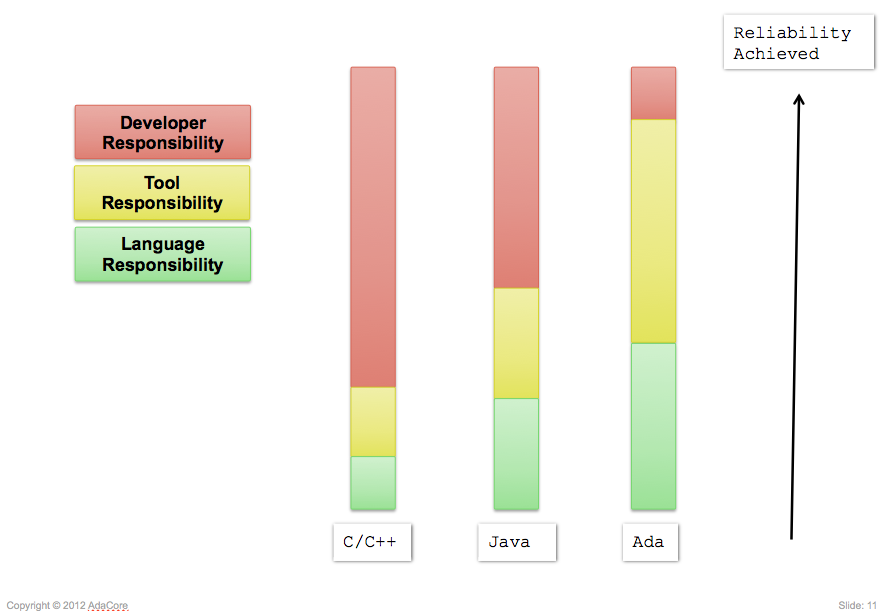
\includegraphics[height=3.5in]{figures/developer_responsibility_in_ada.png}
    	\caption{Developer responsibility in Ada\protect\footnotemark. }    	
    \end{center}
\end{figure}
\footnotetext{http://www.slideshare.net/AdaCore/ada-2012}

SPARK is a programming language and static verification technology designed specifically for the development of high integrity software. It is a "safe" subset of Ada designed to be susceptible to formal methods, accompanied with a set of approaches and tools. SPARK 2005 does not include constructs such as pointers, dynamic memory allocation or recursion \cite{Spark:Article}. Using SPARK, a developer takes a Z specification and performs a stepwise refinement from the specification to SPARK code. For each refinement step a tool is used to produce verification conditions (VC's), which are mathematical theorems. If the VC's can be proved then the refinement step will be known to be valid. However if the VC's cannot be proved then the refinement step may be erroneous\footnote{http://www.dwheeler.com/lovelace/s17s4.htm}. Sample Verification Condition contains checks for:
\begin{itemize}
    \item array index out of range
    \item type range violation
    \item division by zero
    \item numerical overflow
\end{itemize}

[Add more examples where SPARK is used?]
% Barnes' 15.7 where SPARK is used

First version was designed over 20 years ago. SPARK has established a track record of use in embedded and critical systems across a diverse range of industrial domains where safety and security are paramount \cite{Barnes:Book}. 

SPARK provides a significant degree of automation in proving exception freedom \cite{Spark:Article}. SPARK excludes some Ada constructs to make static analysis feasible \cite{Spark:Article}. Additionally SPARK contains tool-set for Software Verification:
\begin{itemize} \itemsep1pt \parskip0pt \parsep0pt
	\item Examiner - analyze code and ensures that it conforms to the SPARK language; also verify program to some extent using Verification Conditions (VC)
	\item Simplifier - simplify Verification Conditions generated by Examiner
	\item ZombieScope - find dead paths, i.e. paths through the code that can never be executed
	\item Proof Checker - prove the Verification Conditions
\end{itemize}

First version of SPARK was based on Ada 83. The second version (SPARK 95) - on Ada 95. SPARK 2005 is based on Ada 2005. It is a subset of Ada 2005 with annotations. The annotation language support flow analysis and formal verification. Annotations are encoded in Ada comments (via the prefix \lstinline{--#}). It makes every SPARK 2005 program, valid Ada 2005 program. 

In real-world applications, the embedded critical components are written in SPARK while the non-critical components are written in Ada.

The crucial part of SPARK Ada are code contracts. Listing \ref{listing:SPARK2005Contracts} presents simple procedure with code contracts. It increments variable given as parameter by 1. The \lstinline{derives} specified variable dependency. It future value depends on its current value. There is precondition saying that the value has to be lower than maximum value of Integer type. There is also post condition, which states that the value of variable (given as parameter) after the procedure execution has to be equal to its previous value incremented by 1.

\begin{lstlisting}[language=ada, frame=single, gobble=0, caption={Sample SPARK procedure with code contracts}, label={listing:SPARK2005Contracts}]
procedure Increment (X : in out Integer);
--# derives X from X;
--# pre X < Integer'Last;
--# post X = X~ + 1;
\end{lstlisting} 


Fundamental SPARK contracts:

\singlespacing
\begin{center}
	\begin{longtable}{| p{1.5in} | p{1.5in} | p{3in} |}
		\caption{Fundamental SPARK annotations}
		\label{table:SparkAnnotations}
		\\
		\hline
		\multicolumn{1}{|c|}{\textbf{SPARK 2005}} & \multicolumn{1}{|c|}{\textbf{SPARK 2014}} & \multicolumn{1}{|c|}{\textbf{Description}} \\ \hline
		\endfirsthead

		\multicolumn{3}{c}%
		{{\bfseries \tablename\ \thetable{} -- continued from previous page}} \\
		\hline 
		\multicolumn{1}{|c|}{\textbf{SPARK 2005}} & \multicolumn{1}{|c|}{\textbf{SPARK 2014}} & \multicolumn{1}{|c|}{\textbf{Description}} \\ \hline
		\endhead

		\hline \multicolumn{3}{|r|}{{Continued on next page}} \\ \hline
		\endfoot

		\hline %\hline
		\endlastfoot

		\begin{lstlisting}
			--# global
		\end{lstlisting} 
		& 
		\begin{lstlisting}[language=ada2012]
			Global
		\end{lstlisting} 
		& 
		list of used global variables within subprogram 

		\\ \hline

		\begin{lstlisting}
			--# derives
		\end{lstlisting} 
		& 
		\begin{lstlisting}[language=ada2012]
			Depends
		\end{lstlisting} 
		& 
		describe dependencies between variables

		\\ \hline

		\begin{lstlisting}
			--# own 
		\end{lstlisting} 
		& 
		\begin{lstlisting}[language=ada2012]
			Abstract_State
		\end{lstlisting} 
		& 
		declare variables defined in package body

		\\ \hline

		\begin{lstlisting}
			--# initializes
		\end{lstlisting} 
		& 
		\begin{lstlisting}[language=ada2012]
			initializes
		\end{lstlisting} 
		& 
		indicates variables, which are initialized

		\\ \hline

		\begin{lstlisting}
			--# inherit
		\end{lstlisting} 
		& 
		not needed
		& 
		allows to access entities of other packages

		\\ \hline

		\begin{lstlisting}
			--# pre
		\end{lstlisting} 
		& 
		\begin{lstlisting}[language=ada2012]
			Pre
		\end{lstlisting} 
		& 
		pre condition

		\\ \hline
		

		\begin{lstlisting}
			--# post
		\end{lstlisting} 
		& 
		\begin{lstlisting}[language=ada2012]
			Post
		\end{lstlisting} 
		& 
		post condition

		\\ \hline
		

		\begin{lstlisting}
			--# assert
		\end{lstlisting} 
		& 
		\begin{lstlisting}[language=ada2012]
			Assert
		\end{lstlisting} 
		& 
		assertion

		\\ \hline
	\end{longtable}
\end{center}
\doublespacing

SPARK 2014\footnote{http://www.spark-2014.org} (based on Ada 2012) is under development. There is partial tool support (in GNAT Programming Studio), but some language features are still not supported. It is worth to mention, that Ada 2012 contains code contracts. Thus SPARK 2014 is just a subset of Ada 2012. \cite{Spark2014:Paper} It contains all features of Ada 2012 except:
\begin{itemize} \itemsep1pt \parskip0pt \parsep0pt
 	\item Access types (pointers)
 	\item Exceptions
	\item Aliasing between variables
	\item Concurrency features of Ada (Tasking) - it's part of SPARK 2014 road-map to include support for tasking in the future, although likely not this year
	\item Side effects in expressions and functions
\end{itemize}

There are no additional constructs such as annotations in SPARK 2014, because now, contracts are part of the language.

Sample mapping from SPARK 2005 to 2014 is shown on table \ref{table:spark2005and2014mapping}. Complete mapping can be found in SPARK 2014 documentation\footnote{http://docs.adacore.com/spark2014-docs/html/lrm/mapping-spec.html} \cite{Spark2014refManual:Online}.

\singlespacing
\begin{table}[!ht]
	\caption{Sample SPARK 2005 to 2014 mapping.}
	\label{table:spark2005and2014mapping}
	\centering
  	\begin{tabular}{ | p{3in} | p{3in} |}
	  	%\multicolumn{1}{c}{\textbf{AADL/BLESS}} & \textbf{SPARK Ada}\\

		\hline
		\multicolumn{1}{|c|}{\textbf{SPARK 2005}} & \multicolumn{1}{|c|}{\textbf{SPARK 2014}} \\ \hline

		\begin{lstlisting}
			--# global in out X, Y;
		\end{lstlisting} 
		& 
		\begin{lstlisting}[language=ada2012]
			with Global  => (In_Out => (X, Y));
		\end{lstlisting} 

		\\ \hline

		\begin{lstlisting}
			--# derives X from Y &
			--#         Y from X;
		\end{lstlisting} 
		& 
		\begin{lstlisting}[language=ada2012]
			Depends => (X => Y,
			            Y => X);
		\end{lstlisting}

		\\ \hline

		\begin{lstlisting}
			--# pre Y /= 0 and
			--#     X > Integer'First;
		\end{lstlisting} 
		& 
		\begin{lstlisting}[language=ada2012]
			with Pre  => Y /= 0 and 
			             X > Integer'First;
		\end{lstlisting}

		\\ \hline

		\begin{lstlisting}
			--# post X = Y~ and Y = X~;
		\end{lstlisting} 
		& 
		\begin{lstlisting}[language=ada2012]
			with Post => (X = Y'Old and Y = X'Old);
		\end{lstlisting} 

		\\ \hline
	\end{tabular}
\end{table}
\doublespacing

SPARK 2014 does not contains Examiner. Instead, proofs are made by gnatPROVE.

The notion of executable contracts in Ada 2012, was inspired by SPARK. The previous example (listing \ref{listing:SPARK2005Contracts}) translated to SPARK 2014 is shown in figure \ref{listing:SPARK2014Contracts}.

\singlespacing
\begin{lstlisting}[language=ada2012, frame=single, gobble=0, caption={Sample SPARK 2014 procedure and Code Contracts}, label={listing:SPARK2014Contracts}]
	procedure Increment (X : in out Integer)
	with Depends => (X => X),
		Pre => (X < Integer'Last),
		Post => (X = X'Old + 1);
\end{lstlisting} 
\doublespacing

It is possible to mix SPARK 2014 with Ada 2012. However, only the part which is SPARK 2014 compliant will be verified. Usually SPARK is used in the most critical parts of Software Systems \cite{Spark:IndustrialExp}. It means, that some part is written in e.g. Ada or C++ and the rest in SPARK. The reason of that is the SPARK limitation and lack of necessity to verify some modules.
% http://docs.adacore.com/spark2014-docs/html/ug/spark_2014.html#mixing-spark-code-and-ada-code

The most popular IDE for SPARK Ada is GNAT Programming Studio\footnote{http://libre.adacore.com/tools/gps}. See section \ref{background:spark:gps}.

There is also plugin for Eclipse: GNATbench\footnote{https://www.adacore.com/gnatpro/toolsuite/gnatbench/} created by AdaCore. 



\subsection{GNAT compiler}
\label{background:spark:gnat}

GNAT compiler is Ada compiler created by AdaCore\footnote{http://www.adacore.com}. It is part of GNU Compiler Collection (GCC). The GNU Compiler Collection includes front ends for C, C++, Objective-C, Fortran, Java, Ada, and Go. It is one of the most popular compiler systems. It is included in all Linux distributions. GNU is open source, published on GNU General Public License. GCC is divided into front end and back end. It allows to create new front end for some language and reuse existing back end.

GNAT supports Ada 2012, Ada 2005, Ada 95 and Ada 83. The front-end and run-time are written in Ada. To make compilation easier, GNAT provides \lstinline{gnatmake} tool. Its take as an argument project file (.gpr) or main file (file, which main procedure) and builds entire program automatically. \lstinline{gnatmake} invokes GCC to perform the actual compilation. It check all dependencies contained in \lstinline{.ali} files. Each invocation of GCC produce object file (\lstinline{.o}) and Ada Library Information file (\lstinline{.ali}). Once compilation is done, \lstinline{gnatmake} invokes \lstinline{gnatbind} tool to check consistency and generate a main program. Then \lstinline{gnatlink} performs linking using binding output and all object files.

GNAT compiler is available for all most popular platforms: Windows, Linux and MacOS. AdaCore, released also GNAT cross-compiler for ARM devices. However, for now, the compilation has to be done on 32-bit Linux platform.


\subsection{GNAT Programming Studio (GPS)}
\label{background:spark:gps}

GNAT Programming Studio (GPS) is Integrated development environment for SPARK Ada. It allows to easily manage and compile SPARK Ada projects using .gpr file. GPS includes set of proving tools. More precisely GUI for setting up their options. Additionally, it enables to create plugins using Python and PyGTK\footnote{http://docs.adacore.com/gps-docs/users\_guide/\_build/html/extending.html}. Sireum Bakar (developed by SAnToS lab) is GPS plugin written in Python and PyGTK. The same with other plugins created by AdaCore like SPARK Examiner or GNATprove.

There are two versions of GPS: free (GPL) and commercial (Pro). There are version for all most popular platforms: Windows, Linux and MacOS.


\subsection{Ravenscar Tasking Subset}
\label{background:spark:ravenscar}

The Ravenscar Profile provides a subset of the tasking facilities of Ada95 and Ada 2005 suitable for the construction of high-integrity concurrent programs \cite{Ravenscar:Online}. RavenSPARK is SPARK subset of the Ravenscar Profile. The Ravenscar Profile is a subset of the tasking model, restricted to meet the real-time community requirements for determinism, schedulability analysis and memory-boundedness, as well as being suitable for mapping to a small and efficient run-time system that supports task synchronization and communication, and which could be certifiable to the highest integrity levels. The concurrency model promoted by the Ravenscar Profile is consistent with the use of tools that allow the static properties of programs to be verified. Potential verification techniques include information flow analysis, schedulability analysis, execution-order analysis and model checking. These techniques allow analysis of a system to be performed throughout its development life cycle, thus avoiding the common problem of finding only during system integration and testing that the design fails to meet its non-functional requirements. \cite{Ravenscar:Article}

Ravenscar profile is available in SPARK 2005, but not yet in SPARK 2014\footnote{http://docs.adacore.com/spark2014-docs/html/lrm/tasks-and-synchronization.html} \cite{Spark2014refManual:Online}. Default profile (sequential) does not enable tasking. In other words, SPARK tools cannot analyze and reason about concurrent programs if Ravenscar profile flag is not provided.

To create a task, the task type has to be declared and task variable of this type. Ravenscar does not allow dynamic task creation. Thus, all tasks have to exists for the full lifetime of the program. \cite{IssuesWithRavenscar:Paper} Tasks can be declared only in packages. Not in subprograms or in other tasks. \cite{Barnes:Book} The priority of each tasks has to be specified by \lstinline{pragma Priority}. [what is priorities range?] Listing \ref{lst:SampleTask} shows sample package with two tasks.

\singlespacing
\begin{lstlisting}[frame=single, gobble=0, caption={Sample tasks}, label={lst:SampleTask}]
	package Some_Pkg
	--# own task t1 : Task1;
	--#     task t2 : Task2;
	is
		task type Task1
		is
			pragma Priority(10);
		end Task1;

		task type Task2
		is
			pragma Priority(9);
		end Task2;

	end Some_Pkg;
\end{lstlisting} 
\doublespacing

Declared tasks have to be implemented in the package body (listing \ref{lst:SampleTaskBody}).

\singlespacing
\begin{lstlisting}[frame=single, gobble=0, caption={Sample tasks body}, label={lst:SampleTaskBody}]
	package body Some_Pkg
	is
		t1 : Task1;
		t2 : Task2;

		task body Task1
		is
		begin
			loop
				-- implementation;
			end loop;
		end Task1;

		task body Task2
		is
		begin
			loop
				-- implementation;
			end loop;
		end Task2;

	end Some_Pkg;
\end{lstlisting} 
\doublespacing

There are two ways to access variable in different tasks:
\begin{itemize}
    \item It has to be protected object
    \item It has to be atomic type
\end{itemize}

Protected object encapsulate variable, in such a way that it is accessible, only through protected subprograms. This mechanism use locking, to ensure atomicity. Protected type declaration is similar to task: specification and body has to be defined. Listing \ref{lst:SampleTasksWithProtectedType} shows sample tasks with protected type \lstinline{Integer_Store}, which enable to share Integer variable between tasks. What is important, protected type has to be declared before tasks, which will use it. Otherwise, it will not be visible for them.

\singlespacing
\begin{lstlisting}[frame=single, gobble=0, caption={Sample tasks with protected object}, label={lst:SampleTasksWithProtectedType}]
	package Some_Pkg
	--# own protected Shared_Var : Integer_Store (Priority => 11);
	--#     task t1 : Task1;
	--#     task t2 : Task2;
	is
	    protected type Integer_Store
	    is
	        pragma Priority (11);

	        function Get return Integer;
	        --# global in Integer_Store;

	        procedure Put(X : in Integer);
	        --# global out Integer_Store;
	        --# derives Integer_Store from X;
	    private
	        TheStoredData : Integer := 0;
	    end Integer_Store;

	    task type Task1
	      --# global out Shared_Var;
	    is
	        pragma Priority(10);
	    end Task1;

	    task type Task2
	      --# global in Shared_Var;
	    is
	        pragma Priority(9);
	    end Task2;

	end Some_Pkg;
\end{lstlisting}
\doublespacing

Protected type body also has to be defined in package body (listing \ref{lst:SampleTasksWithProtectedTypeBody}).

\singlespacing
\begin{lstlisting}[frame=single, gobble=0, caption={Sample tasks with protected object body}, label={lst:SampleTasksWithProtectedTypeBody}]
	package body Some_Pkg
	is
	    Shared_Var : Integer_Store;
	    t1 : Task1;
	    t2 : Task2;

	    protected body Integer_Store is
	        function Get return Integer
	        --# global in TheStoredData;
	        is
	        begin
	            return TheStoredData;
	        end Get;

	        procedure Put(X : in Integer)
	        --# global out TheStoredData;
	        --# derives TheStoredData from X;
	        is
	        begin
	            TheStoredData := X;
	        end Put;
	    end Integer_Store;

	    task body Task1
	    is
	    begin
	        loop
	            Shared_Var.Put(5);
	        end loop;
	    end Task1;

	    task body Task2
	    is
	        Local_Var : Integer;
	    begin
	        loop
	            Local_Var := Shared_Var.Get;
	        end loop;
	    end Task2;

	end Some_Pkg;
\end{lstlisting} 
\doublespacing

\lstinline{Task1} is writing to \lstinline{Shared_Var} and \lstinline{Task2} is reading \lstinline{Shared_Var}. The highest priority is assigned to protected object, to ensure atomicity during operations on it. The lowest priority is assigned to \lstinline{Task2}, which is reading \lstinline{Shared_Var}. Reading is usually less expensive operation than writing. Thus, to avoid starvation, \lstinline{Task1} has higher priority than \lstinline{Task2}. Notice, that \lstinline{Shared_Var} is declared in package body, but refined in package specification.

Protected variables may not be used in proof contexts. Thus, if we try to use protected variable in proofs (pre- or postcondition), then SPARK Examiner returns following error: \lstinline{Semantic Error 940 - Variable is a protected own variable. Protected variables may not be used in proof contexts.}. Formal reasoning about interactions and especially temporal properties require other techniques such as model checking and lie outside the scope of SPARK \cite{Barnes:Book}. To preserve opportunity to use pre- and postconditions, atomic types have to be used.

To declare atomic type, \lstinline{pragma Atomic} has to be used. However, there is restriction, that \lstinline{pragma Atomic} cannot be applied to predefined type such as Integer. Thus, custom type has to be defined. It can be just rename of Integer. Then \lstinline{pragma Atomic} can be applied on this type. Listing \ref{lst:SampleTasksWithAtomicType} presents previous example with atomic types instead of protected objects.

\singlespacing
\begin{lstlisting}[frame=single, gobble=0, caption={Sample tasks with atomic type}, label={lst:SampleTasksWithAtomicType}]
	package Some_Pkg
	--# own Shared_Var;
	--#     task t1 : Task1;
	--#     task t2 : Task2;
	--# initializes Shared_Var;
	is
	    type Int32 is new Integer;
	    
	    task type Task1
	      --# global out Shared_Var;
	    is
	        pragma Priority(10);
	    end Task1;

	    task type Task2
	      --# global in Shared_Var;
	    is
	        pragma Priority(9);
	    end Task2;

	end Some_Pkg;

	package body Some_Pkg
	is    
	    Shared_Var : Int32 := 0;
	    t1 : Task1;
	    t2 : Task2;

	    task body Task1
	    is
	    begin
	        loop
	            Shared_Var := 5;
	        end loop;
	    end Task1;

	    task body Task2
	    is
	        Local_Var : Integer;
	    begin
	        loop
	            Local_Var := Integer(Shared_Var);
	        end loop;
	    end Task2;

	end Some_Pkg;
\end{lstlisting}
\doublespacing

It is important to mention, that \lstinline{pragma atomic} does not guaranty atomicity. In most cases, atomic types should not be used for tasking. Instead, protected types should be used. When an object is declared as atomic, it just means that it will be read from or written to memory atomically. The compiler will not generate atomic instructions or memory barriers when accessing to that object. \lstinline{pragma atomic} force compiler, to:
\begin{itemize}
	\item check if architecture guarantees atomic memory loads and stores,
	\item disallow some compiler optimizations, like reordering or suppressing redundant accesses to the object
\end{itemize}
% http://en.wikibooks.org/wiki/Ada_Programming/Pragmas/Atomic

Another important thing in tasking is Time library: \lstinline{Ada.Real_Time}. It allows to run task periodically, using \lstinline{delay until} statement, which suspends task until specified time. To use \lstinline{delay} in the task, it has to be declared in \lstinline{declare} annotation: \lstinline{--# declare delay;} \cite{Barnes:Book}.

Details about tasking in SPARK are well described in Chapter 8 of Barnes' book \cite{Barnes:Book}. The "Guide for the use of the Ada Ravenscar profile in high integrity systems" \cite{Ravenscar:Article} and the official Ravenscar Profile documentation (which includes examples) \cite{Ravenscar:Online} might be useful as well. The limitations of Tasking in SPARK are reviewed in Audsley's and Welllings' paper \cite{IssuesWithRavenscar:Paper}.



\section{SPARK Ada Verification}
\label{background:sparkverification}

%http://docs.adacore.com/sparkdocs-docs/

The goal of software verification is to assure software correctness and lack of errors. There are two types of verification:
\begin{itemize}
	\item dynamic - performed during the execution of software, e.g. unit tests
	\item static - achieved by formal methods, mathematical calculations and logical evaluations
\end{itemize}

Dynamic verification starts with a set of possible test cases, simulates the system on each input, and observes the behavior. In general, it does not cover all possible executions. On the other hand, static verification establishes correctness for all possible execution sequences.

Techniques for Static Verification:
\begin{itemize}
	\item Formal verification: prove mathematically that the program is correct - this can be difficult for large programs.
	\item Correctness by construction: follow a well- defined methodology for constructing programs.
	\item Model checking: enumerate all possible executions and states, and check each state for correctness.
\end{itemize}

\begin{figure}[ht]%t=top, b=bottom, h=here
    \begin{center}
    	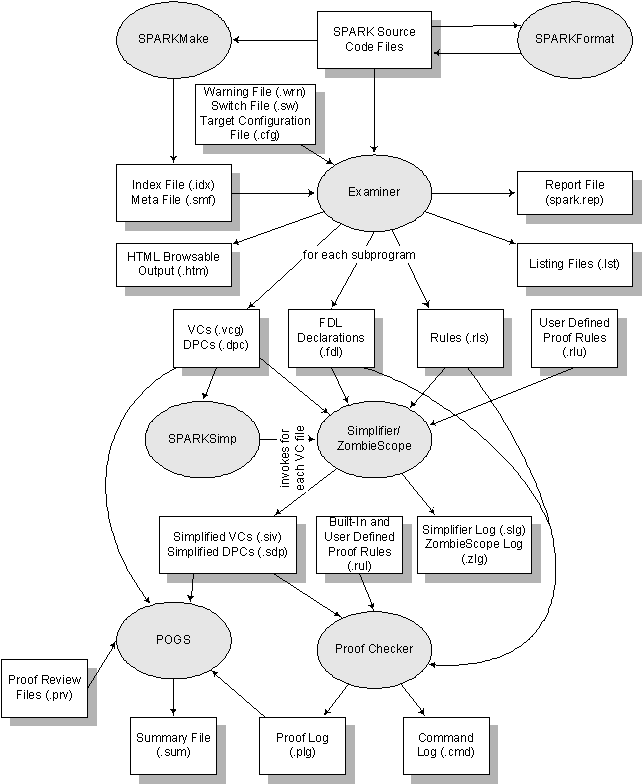
\includegraphics[height=0.6\textheight]{figures/spark-tools.png}
    	\caption{Relationship of the Examiner and Proof Tools\protect\footnotemark.}
    \end{center}
    \label{figure:spark-tools}
\end{figure}
\footnotetext{http://docs.adacore.com/sparkdocs\-docs/Examiner\_UM.htm}

SPARK consists of a verification toolset:
\begin{itemize}
	\item SPARKMake - generates index file (.idx) and meta file (.smf)
	\item Examiner - check syntax, generates Verification Conditions (VCs) and Dead Path Conjectures (DPCs), and discharge (prove them)
	\item Simplifier - simplify and discharge VCs, which are not discharged by Examiner
	\item ZombieScope - find dead paths
	\item ViCToR - translate VCs and DPCs to format acceptable by SMT solver and prove correctness using specified SMT solver
	\item SPARKSimp - runs Simplifier or/and ZombieScope
	\item POGS - produces verification report
	\item Proof Checker - discharge VCs or DPCs not discharged by Examiner and Simplifier
\end{itemize}

Relationships between tools and verification flow is presented on figure \ref{figure:spark-tools}. SPARK proof tools use FDL as the modeling language. 


\subsection{SPARK Examiner}
\label{verification:examiner}

The main SPARK verification tool is Examiner. It supports several levels of analysis:
\begin{itemize}
	\item checking of SPARK language syntactic and static semantic rules
	\item data flow analysis
	\item data and information flow analysis
	\item formal program verification via generation of verification conditions
	\item proof of absence of run-time errors
	\item dead path analysis
\end{itemize}

There is also an option to make the Examiner perform syntax checks only. Using this option on a source file does not require access to any other units on which the file depends, so files can be syntax checked on an individual basis. This allows any syntax errors to be corrected before the file is included in a complex examination. This option must only be used as a pre-processor: the absence of syntax errors does NOT indicate that the source text is a legal SPARK program. \cite{Examiner:Online} [THIS PART IS COPY AND PASTE FROM Examiner doc - is it ok?]

[Put here some examples? E.g.: method without contract, examine, add specification, pass Examiner.]

Examiner can perform data and information analysis of Ravenscar programs in exactly the same manner as for sequential programs \cite{Ravenscar:Online}. Unfortunately it does not allow protected objects in proof annotations (pre- and post-conditions). As mentioned in section \ref{background:spark:ravenscar}.

When some parts of the system are written in full Ada (with non-valid SPARK constructs), then Examiner returns error. Ada parts can be excluded from Examiner analysis using \lstinline{--# hide} annotation. Then, only warning \lstinline{10 - The body of subprogram Main is hidden - hidden text is ignored by the Examiner.} is returned by Examiner.

Examiner use SPARK index file (.idx) - generated by \lstinline{SPARKMake} tool -  to locate files necessary for verification. \cite{Barnes:Book}

Examiner can be used with \lstinline{spark} command and appropriate flags described in Examiner Manual \cite{Examiner:Online}.

%http://docs.adacore.com/sparkdocs-docs/SPARK_GPS.htm

To use Examiner in GNAT Programming Studio:
\begin{itemize}
	\item Run SPARK Make: right click on project / SPARK / SPARK Make (figure \ref{figure:sparkmake})
	\item Set SPARK index file (to spark.idx generated by SPARKMake) (figure \ref{figure:examinerproperties})
	\item (optionally) set configuration file (Standard.ads)
	\item Choose appropriate version of SPARK (95 or 2005)
	\item Choose mode: Sequential (for single tasking programs) or Ravenscar (for multitasking programs)
\end{itemize}

\begin{figure}[ht]%t=top, b=bottom, h=here
    \begin{center}
    	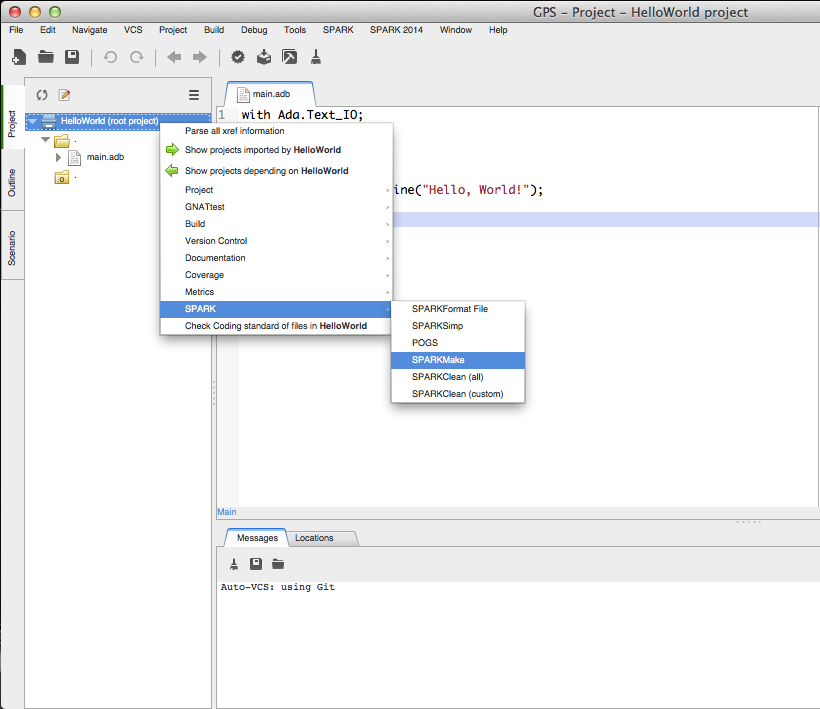
\includegraphics[width=3in]{figures/SPARKMake.png}
    	\caption{Run SPARK Make}
    \end{center}
    \label{figure:sparkmake}
\end{figure}

\begin{figure}[ht]%t=top, b=bottom, h=here
    \begin{center}
    	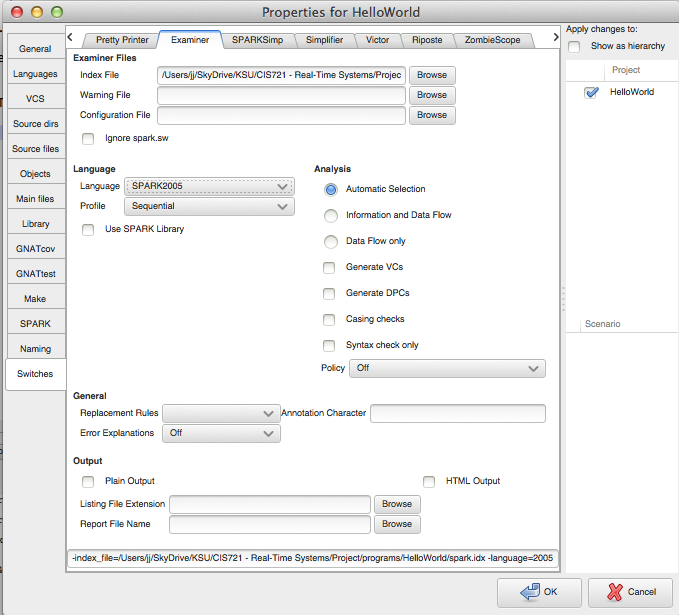
\includegraphics[width=3in]{figures/Properties-Switches-Examiner.png}
    	\caption{Examiner Properties}
    \end{center}
    \label{figure:examinerproperties}
\end{figure}

To generate verification conditions (VCs), the \lstinline{-vcg} switch has to be used. It can be set in GNAT Programming Studio (Project / Edit project properties / Switches / Examiner / Generate VCs).
In addition to verification conditions, Examiner can check dead path conjectures (DPCs). It checks, whether all of the program is useful. To generate dead path conjectures, the \lstinline{-dpc} switch has to be used. It can be also set in GNAT Programming Studio (Project / Edit project properties / Switches / Examiner / Generate DPCs).


\subsubsection{Flow analysis}
\label{verification:examiner:flowanalysis}
%http://www.cs.swan.ac.uk/~csetzer/lectures/critsys/09/critsysfinal2.pdf
There are two types of flow analysis:
\begin{itemize}
	\item Data flow analysis:
	\begin{itemize}
		\item Checks input/output behavior of parameters and variables.
		\item Checks initialization of variables.
		\item Checks that changed and imported variables are used later (possibly as output variables).
	\end{itemize}
	\item Information flow analysis - verifies interdependencies between variables.
\end{itemize}

In data flow analysis, Examiner checks if input parameters are not modified, but used at least once (in at least one branch of program). In the same factor, output parameters cannot be read (before initialization) and has to be initialized (in all branches of program). Input/output parameters has to be both read and write (changed). In similar way, Examiner verify the global variables (specified in annotations). Functions can use only input parameters and can only read global variables. Therefore functions do not have side effects. 

Global variables defined in package body (thus private) has to be declared by \lstinline{--# own} annotation in package specification. If variable is also initialized, \lstinline{--# initializes} annotation has to be used. In Ada, to use package in another package, \lstinline{with} clause has to be used. In SPARK Ada, additionally \lstinline{--# inherits} annotation has to be specified.

In information flow analysis, dependencies between variables are analyzed. These dependencies are specified by \lstinline{--# derives} annotation.


\subsubsection{Verification conditions}
\label{verification:examiner:vc}

To generate verification conditions, two kinds of annotations are relevant for Examiner:
\begin{itemize}
	\item pre-conditions: \lstinline{--# pre}
	\item post-conditions: \lstinline{--# post}
\end{itemize}

Notion of pre- and post-conditions represents Hoare logic. More precisely, Hoare triple: 

\begin{equation} \label{eq:hoare_triple}
	\{P\} C \{Q\}
\end{equation}

P and Q are assertions. C is a command (action) performed between them. P is pre-condition and Q is post-condition.

Additionally, assertions (\lstinline{--# assert}) and checks (\lstinline{--# check}) can be specified in procedure body. Then additional verification conditions are generated.

Functions does not have side effects (as stated in \ref{verification:examiner:flowanalysis}), thus only pre-condition can be applied. However, there is annotation \lstinline{--# return}, which specify function return value.

Verification conditions are generated depended on number of paths in subprogram. Analysis are perform backwards, in other words: we start from post-conditions and consider what must holds before. Flow analysis is well described in chapter 11 of Barnes' book \cite{Barnes:Book}.

If pre-conditions are not present, then the formula expresses that the post-condition holds always.



\subsection{SPARK Simplifier}
\label{verification:simplifier}

Simplifier, simplify verification conditions (VCs) generated by Examiner. It can also discharge (prove correctness) of those VCs, which are not proved by Examiner. \cite{Simplifier:Online} It takes as input .vcg files, .fdl files for its data declarations and - if available - proof-rule files (.rls, .rlu). Then it generates .siv files (simplified VCs) and .slg files (details about simplification, which has been done).



\subsection{ZombieScope}
\label{verification:zombiescope}

ZombieScope is a SPARK tool, that analyses SPARK code to find dead paths, i.e. paths through the code that can never be executed.

Program, which contains dead paths may not necessarily be incorrect, but a dead path is an indication of a potential code issue.

ZombieScope reads .dpc files generated by the Examiner. In order to generate dead path conjectures, -dpc flag has to be used or 'Generate DPCs' option has to be checked in Examiner options, in GPS. It reads also .fdl files for its data declarations and the .rls file for proof-rules if present. ZombieScope generates two output files: .sdp (dead path summary) file and .zlg file (details about underlying contradiction search performed). ZombieScope is invoked by SPARKSimp by default and the summary file generated by POGS includes information about the dead path analysis.


\subsection{ViCToR}
\label{verification:victor}

ViCToR is a tool to translate SPARK verification conditions (VCs), as generated by the Examiner, into SMT-LIB (file format used to communicate with SMT solvers). \cite{Victor:Online} SMT (Satisfiability Modulo Theories) solver is a tool for verification and proving the correctness of programs. ViCToR is integrated with SPARKSimp (by -victor flag) and POGS.


\subsection{Proof Checker}
\label{verification:proofchecker}

% Barnes' book: 12.12
Proof Checker is advanced verification tool, which require considerable experience in verification of SPARK programs. It is interactive program, which enables the user to direct the Checker to explore the use of various strategies and rules on the condition to be proved. Proof Checker can keep a log of the progress of a proof in \lstinline{plg} file. It also keep command record in \lstinline{cmd} file.


\subsection{SPARKSimp Utility}
\label{verification:sparksimp}
SPARKSimp is a simple "make" style tool for the SPARK analysis tools. Currently, it supports the Simplifier, ZombieScope and ViCToR. It applies the Simplifier (and ViCToR, if requested, please see the Victor\_Wrapper user manual \cite{Victor:Online} for more information) to all .vcg files and ZombieScope to all .dpc files it finds in a directory tree. \cite{SPARKSimp:Online} 


\subsection{Proof Obligation Summarizer (POGS)}
\label{verification:pogs}

The Proof ObliGation Summarizer tool (POGS) reads and understands the structure of the verification condition files (.vcg), their simplified version (.siv) and dead path conjectures files (.dpc). It reports the status of proofs and dead path analyses in a human-readable, text form. \cite{POGS:Online} 


\subsection{AUnit}
\label{background:spark:aunit}

AUnit is Unit Test Framework for Ada language. It can be also applied for verify SPARK Ada programs. Is was created based on Java JUnit (created by Kent Beck, Erich Gamma) and C++ CppUnit (created by M. Feathers, J. Lacoste, E. Sommerlade, B. Lepilleur, B. Bakker, S. Robbins) unit test frameworks \cite{AUnitCookbook:Online}. Similar like mentioned frameworks it enable simple test cases testing, fixtures, suites and provides reporting \cite{AUnitTutorials:Online}.

GNAT Programming Studio can generate test cases skeleton for all subprograms. It can be generated using Tools -> GNATtest -> Generate unit test setup. This generator creates new project with AUnit tests. Project for which tests are generated is referenced in new generated project. In order to run tests, the test project has to be opened in GNAT Programming Studio. The project is created in \lstinline{[project_dir]/gnattest/harness/test_[proj_name].gpr}. It generates empty (not implemented) test for each subprogram in project. To add/edit/remove tests or rename names, three files has to be edited:

\begin{itemize}
    \item \lstinline{[some_package]-test_data-tests.ads}
    \item \lstinline{[some_package]-test_data-tests.adb}
    \item \lstinline{[some_package]-test_data-tests-suite.adb}
\end{itemize}

Test has to be declared in \lstinline{[some_package]-test_data-tests.ads} and implemented in \lstinline{[some_package]-test_data-tests.adb}. Then it has to be added to test suite in \lstinline{[some_package]-test_data-tests-suite.adb} file.

Tests can be also created manually. Then the AUnit distribution has to be referenced in project file and test cases has to be implemented.


\subsection{Sireum Bakar}
\label{background:spark:sireum}

Sireum\footnote{http://www.sireum.org/} is a long-term research conducted by SAnToS lab at Kansas State Univeristy. Its goal is to develop an over-arching software analysis platform that incorporates various static analysis techniques such as data-flow framework, model checking, symbolic execution, abstract interpretation, and deductive reasoning techniques (e.g., using weakest precondition calculation). It can be used to build various kinds of software static analyzers for different kinds of properties. 

It uses the Pilar language as intermediate representation. Any language which can be translated to Pilar can be analyzed by Sireum. For now, there is translator for SPARK and Java.

Bakar is a toolset for analyzing SPARK Ada programs (Bakar means “spark” in Indonesian).

Sireum Bakar currently includes:
\begin{itemize}
	\item Alir
	\item Kiasan
\end{itemize}


\subsubsection{Bakar Kiasan}

Bakar Kiasan \cite{Kiasan:Paper} is a fully automated tool for verifying functional behaviors of SPARK programs specified as software contract (Kiasan means “symbolic” in Indonesian). Kiasan use symbolic execution technique. It provides various helpful feedback including generation of counter example for contract refutation, test cases for an evidence of contract satisfaction, verification reports, visual graphs illustrating pre/post states of SPARK procedures/functions, etc. It is much easier for analysis by developer than e.g. .vcg files generated by SPARK Examiner.

There exists Kiasan Plug-in for GNAT Programming Studio (GPS). Version 1, for GPS 5, supports SPARK 2005. Version 2, for GPS 6, which supports 2014 is under development. Both plug-ins are created by author of this thesis in Python and PyGTK. There is also plug-in for Eclipse, but only for SPARK 2005 programs.

Bakar Kiasan does not support Ravenscar profile. Thus, it can be used only for sequential programs. Figure \ref{figure:kiasan-sample} depicts sample Kiasan analysis result. Kiasan window has two parts: list of units (packages and subprograms) and analysis cases with pre and post states. Every unit has associated statistics:
\begin{itemize}
	\item T\# - Test cases (expected behavior)
	\item E\# - Exception cases (unexpected behavior)
	\item Instruction coverage - amount of code covered by Kiasan analysis
	\item Branch coverage - number of branches covered by analysis (0\% in 100\% instruction coverage means, that there is no branches in analyzed unit)
	\item Time is which analyze was performed
\end{itemize}

After double click on some unit, code which is executed during execution of this unit is highlighted. Additionally below the list of units there is a combo box, which contains all test cases associated with selected (by double click) unit. Once, some case is selected, code coverage equivalent to this test case is highlighted. Additionally, below combo box, there are states of unit execution. On the left hand side, there is pre-state, and on the right hand side there post-state of analysis. Variables with red font color, in post-state, are those which are changed in result of unit execution. The new created variables (during unit execution) are blue, but there are not present in figure \ref{figure:kiasan-sample}.

\begin{figure}[ht]%t=top, b=bottom, h=here
    \begin{center}
    	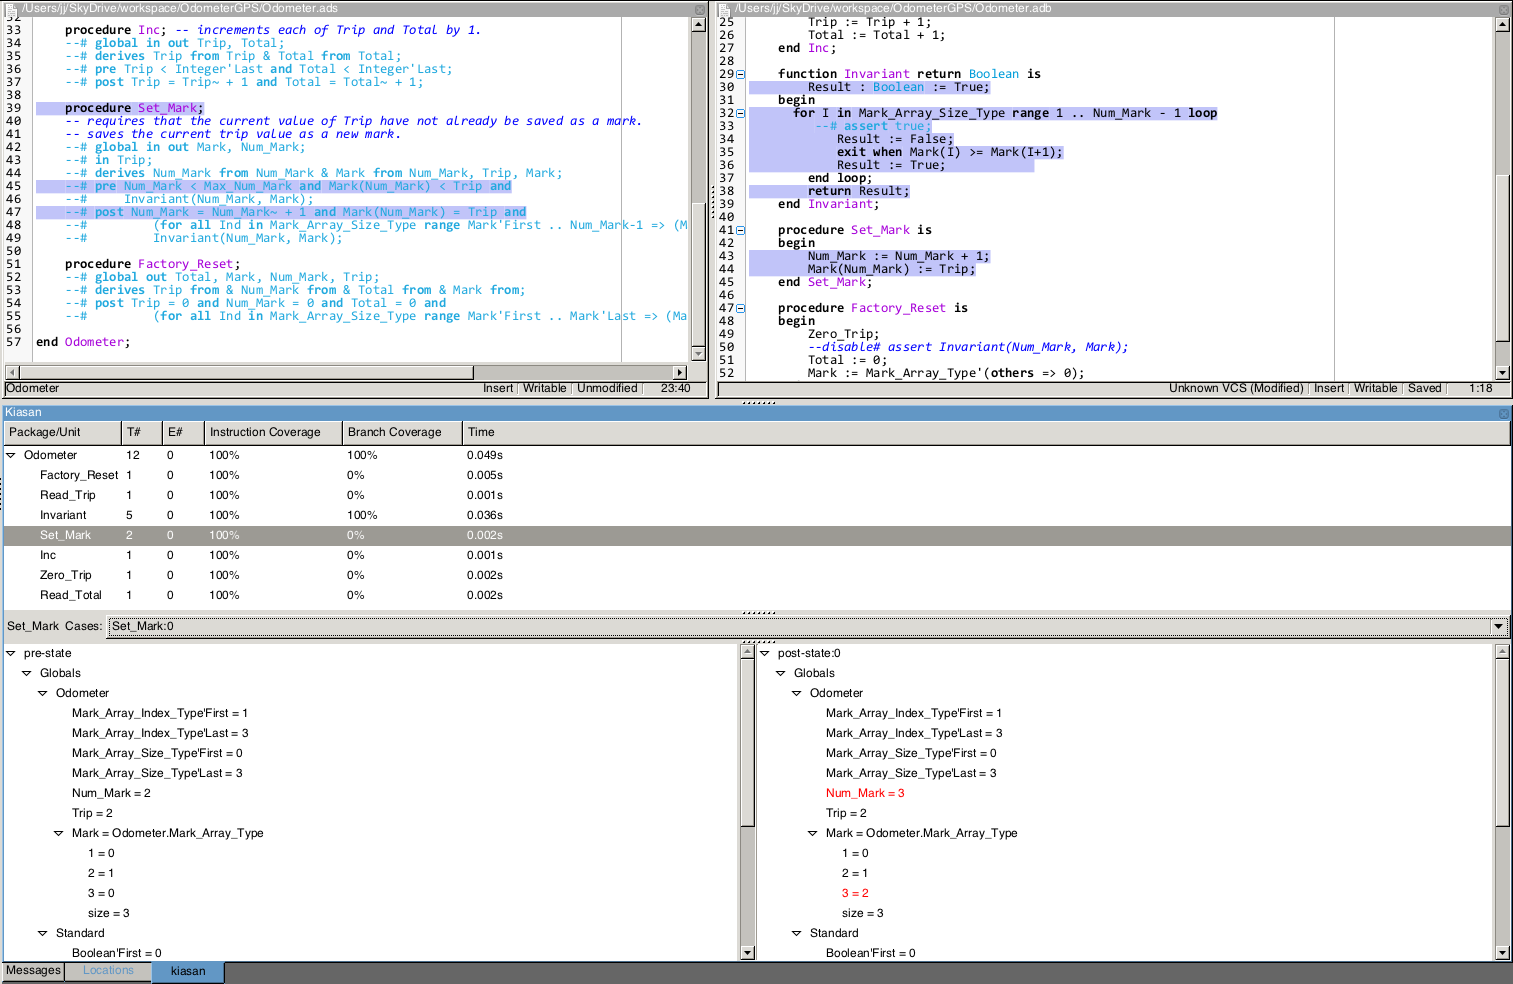
\includegraphics[width=1\textwidth]{figures/kiasan-sample.png}
    	\caption{Bakar Kiasan report}
    \end{center}
    \label{figure:kiasan-sample}
\end{figure}

Bakar Kiasan is useful especially, for solving verification issues. It can generate counter examples, which help to fix the code.
[add screenshot with error case and discuss result?]


\subsubsection{Bakar Alir}
Alir is an information flow analysis tool for reasoning about SPARK's derive clauses/information flow (Alir means "flow" in Indonesian). Alir visualizes information flows to ease engineers in understanding information dependencies crucial for specifying and verifying SPARK's derive clauses. It provides various configurable intra-procedural and inter-procedural analyses. The inter-procedural analyses are control flow analysis, reaching definition analysis and data dependence analysis. The inter-procedural analysis in Alir includes building, System Dependence Graph (SDG), slicing and chopping on SDG. \cite{Hari:Thesis}


\subsection{GNAT Prove}
\label{background:spark:gnatprove}
GNATprove \footnote{http://www.open-do.org/projects/hi-lite/gnatprove/} is a formal verification tool for SPARK 2014 programs. It interprets SPARK Ada annotations exactly like they are interpreted at run time during tests.
% http://docs.adacore.com/spark2014-docs/html/ug/gnatprove.html
% only for SPARK 2014


\section{AADL/BLESS to SPARK Ada code generation}
\label{background:codegen}
The ultimate goal of long term research, this thesis is part of, is AADL (with BLESS) to SPARK Ada translation.


\subsection{Ocarina}
\label{background:codegen:ocarina}
Ocarina \cite{Ocarina:Paper,Ocarina:Paper} generates code from an AADL architecture model to an Ada application running on top of PolyORB framework. In this context, PolyORB acts as both the distribution middleware and execution runtime on all targets supported by PolyORB.
It generate Ada 2005 and C code.
Since mid-2009, Telecom ParisTech is no longer involved in Ocarina, and is developing another AADL tool-chain, based on Eclipse, codenamed RAMSES \cite{Ocarina:About:Online}.

examples on github

run:
ocarina -x scenario.aadl



\subsection{Ramses}
\label{background:codegen:ramses}
% very shortly
RAMSES is a model transformation framework dedicated to the refinement of AADL models. It contains code generation plug-in.
% http://www.aadl.info/aadl/downloads/committee/feb2013/presentations/RAMSES_status_2013_06_02_format.pdf
% https://wiki.sei.cmu.edu/aadl/index.php/OSATE_2_on_the_command-line